\section*{1.}

\subsection*{A.}

The signal is created, sampled and then stored in Listing~\ref{lst:1a}.
Some utility variables and functions used are defined in Listing~\ref{lst:utils}.
Libraries used are imported in Listing~\ref{lst:libs}.

\lstinputlisting[
  language=Python,
  firstline=15,
  lastline=26,
  label={lst:1a},
  caption={1A: Sampling and writing audio of signal}]
  {code.py}

\lstinputlisting[
  language=Python,
  firstline=7,
  lastline=11,
  label={lst:utils},
  caption={Utility variables and functions}]
  {code.py}

\lstinputlisting[
  language=Python,
  firstline=1,
  lastline=5,
  label={lst:libs},
  caption={Python libraries}]
  {code.py}

\subsection*{B.}

Figure~\ref{fig:1b} displays the power spectrum of y.
As seen from the figure, the peaks correspond to the frequencies in the signal.
The code for computing the DFT and plotting the spectrum is shown in Listing~\ref{lst:1b}.

\begin{figure}[H]
  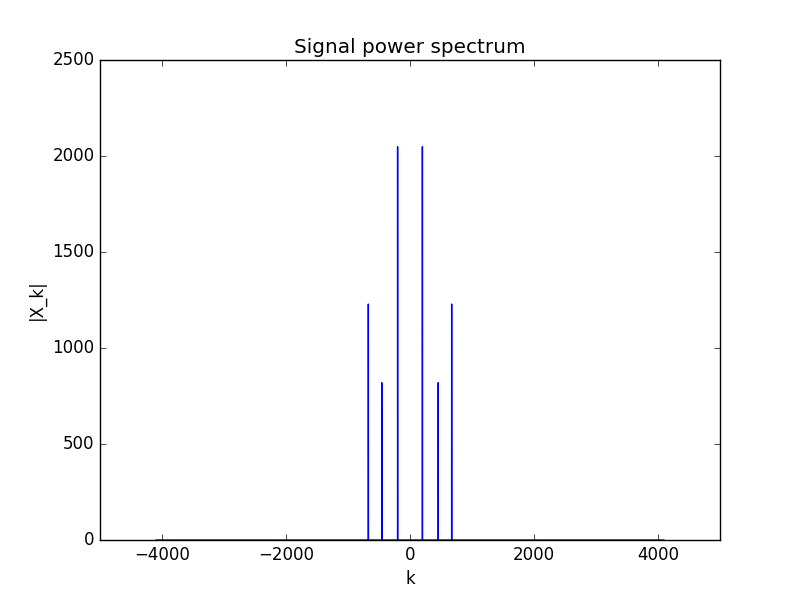
\includegraphics[width=\textwidth]{1b}
  \caption{Signal y power spectrum}
  \label{fig:1b}
\end{figure}

\lstinputlisting[
  language=Python,
  firstline=28,
  lastline=35,
  label={lst:1b},
  caption={Signal y power spectrum}]
  {code.py}

\subsection*{C.}

Listing~\ref{lst:filter-dft} creates the filter DFT as defined in the task.
Figure~\ref{fig:1c-power} displays the power spectrum of this filter, plotted by Listing~\ref{lst:filter-power}.
The filter DFT is inverse DFT transformed in Listing~\ref{lst:filter-idft} to get the filter which is plotted in Figure~\ref{fig:1c-filter} by Listing~\ref{lst:filter-plot}.
All the components of the filter are nonzero, as calulated by Listing~\ref{lst:nonzero}.

\lstinputlisting[
  language=Python,
  firstline=37,
  lastline=43,
  label={lst:filter-dft},
  caption={Filter DFT (H)}]
  {code.py}

\lstinputlisting[
  language=Python,
  firstline=46,
  lastline=51,
  label={lst:filter-power},
  caption={H power spectrum}]
  {code.py}

\begin{figure}[H]
  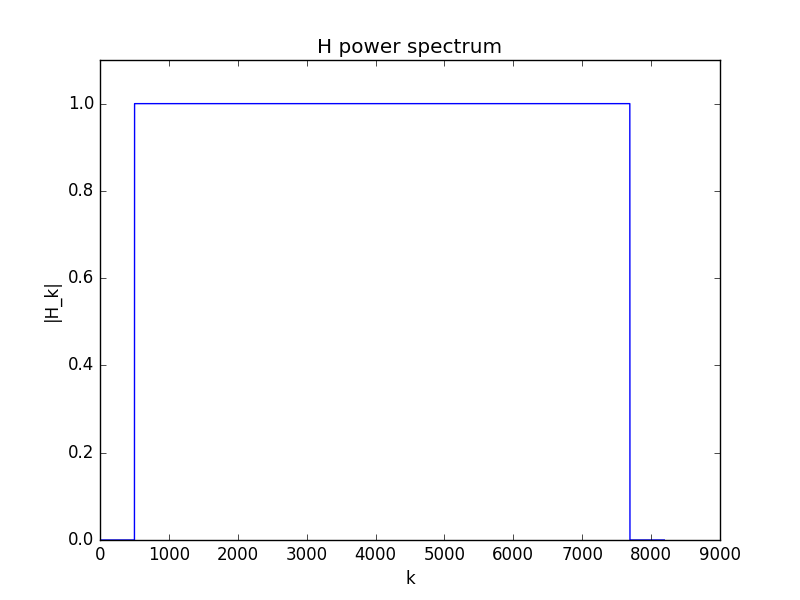
\includegraphics[width=\textwidth]{1c_power}
  \caption{H power spectrum}
  \label{fig:1c-power}
\end{figure}

\lstinputlisting[
  language=Python,
  firstline=44,
  lastline=44,
  label={lst:filter-idft},
  caption={H inverse DFT}]
  {code.py}

\lstinputlisting[
  language=Python,
  firstline=53,
  lastline=58,
  label={lst:filter-plot},
  caption={h filter signal}]
  {code.py}

\begin{figure}[H]
  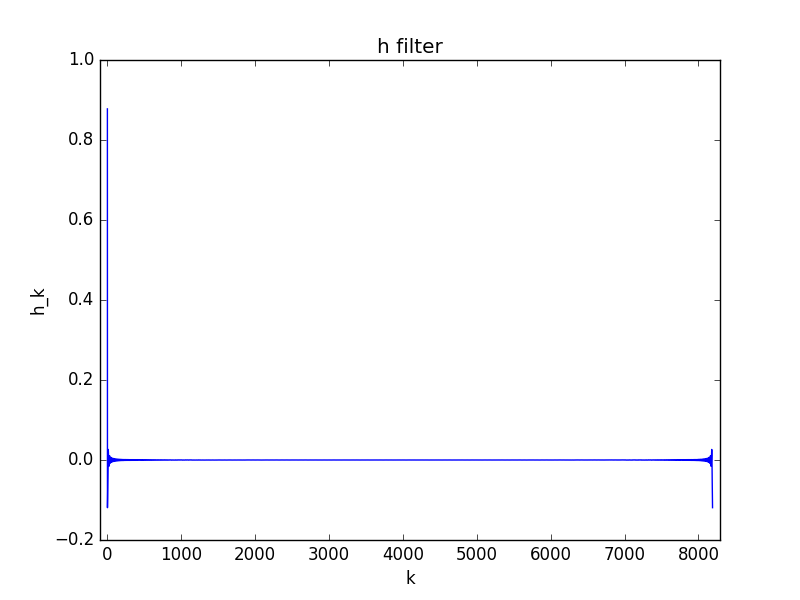
\includegraphics[width=\textwidth]{1c_signal}
  \caption{h filter signal}
  \label{fig:1c-filter}
\end{figure}

\lstinputlisting[
  language=Python,
  firstline=60,
  lastline=61,
  label={lst:nonzero},
  caption={Nonzero count of signal}]
  {code.py}

\subsection*{D.}

The signal y was filtered with h by conjugating y and h in Listing~\ref{lst:conj}, then written to an audio file in Listing~\ref{lst:conj-write}.
One could clearly hear only the highest frequency.
Figure~\ref{fig:filtered} displays the power spectrum of the filtered signal.
It was created by the code in Listing~\ref{lst:filtered-plot}.
The spectrum shows that only one frequency remains.

\lstinputlisting[
  language=Python,
  firstline=63,
  lastline=63,
  label={lst:conj},
  caption={Filtering signal y with filter h by conjugation}]
  {code.py}

\lstinputlisting[
  language=Python,
  firstline=64,
  lastline=64,
  label={lst:conj-write},
  caption={Writing the filtered signal}]
  {code.py}

\lstinputlisting[
  language=Python,
  firstline=66,
  lastline=70,
  label={lst:filtered-plot},
  caption={Plotting the power spectrum of the filtered signal}]
  {code.py}

\begin{figure}[H]
  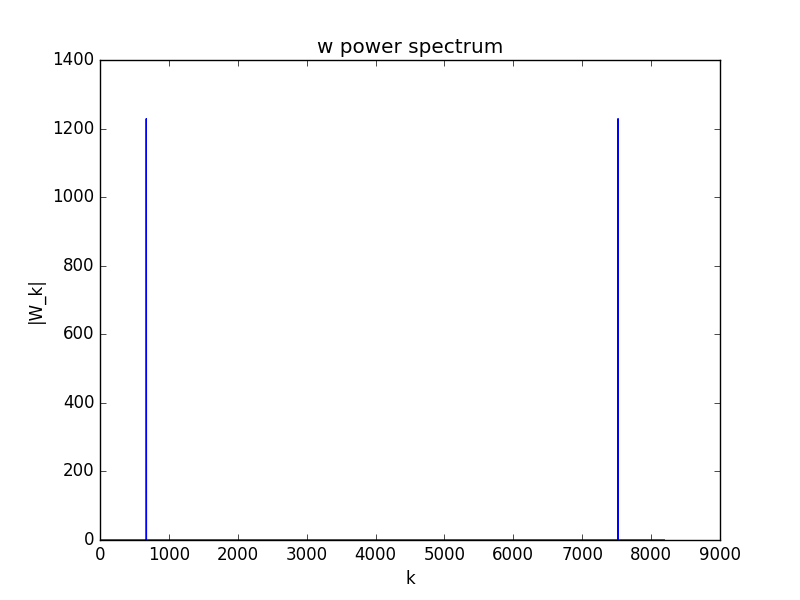
\includegraphics[width=\textwidth]{1d}
  \caption{Power spectrum of filtered signal}
  \label{fig:filtered}
\end{figure}

\section*{2.}

\subsection*{A.}

The signal is sampled, transformed by DFT and plotted in Listing~\ref{lst:2a}.
The plot is seen in Figure~\ref{fig:2a}.
From the plot one can clearly see two frequencies which should be 137 and 147.
The first frequency is much stronger than the second, which matches with the amplitudes in the signal.

\lstinputlisting[
  language=Python,
  firstline=74,
  lastline=90,
  label={lst:2a},
  caption={Signal sampling and DFT magnitude plot}]
  {code.py}

\begin{figure}[H]
  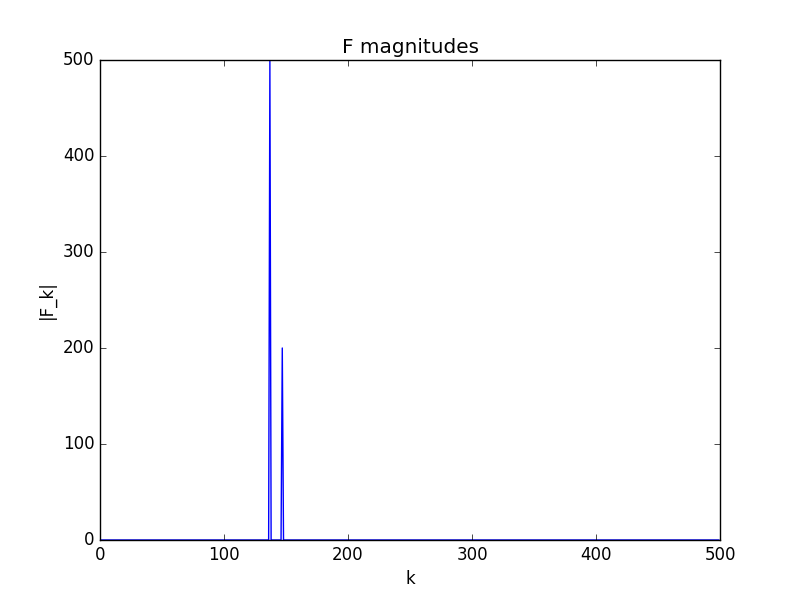
\includegraphics[width=\textwidth]{2a}
  \caption{DFT magnitudes of signal}
  \label{fig:2a}
\end{figure}

\subsection*{B.}

Listing~\ref{lst:window} constructs a windowed version of the signal with a size of 200 and plots the magnitudes of the first 100 components of the DFT.
The plot can be seen in Figure~\ref{fig:window}.
The two frequencies still have distinguishable spikes, but they are much wider than earlier.

\lstinputlisting[
  language=Python,
  firstline=92,
  lastline=99,
  label={lst:window},
  caption={Window DFT and plot}]
  {code.py}

\begin{figure}[H]
  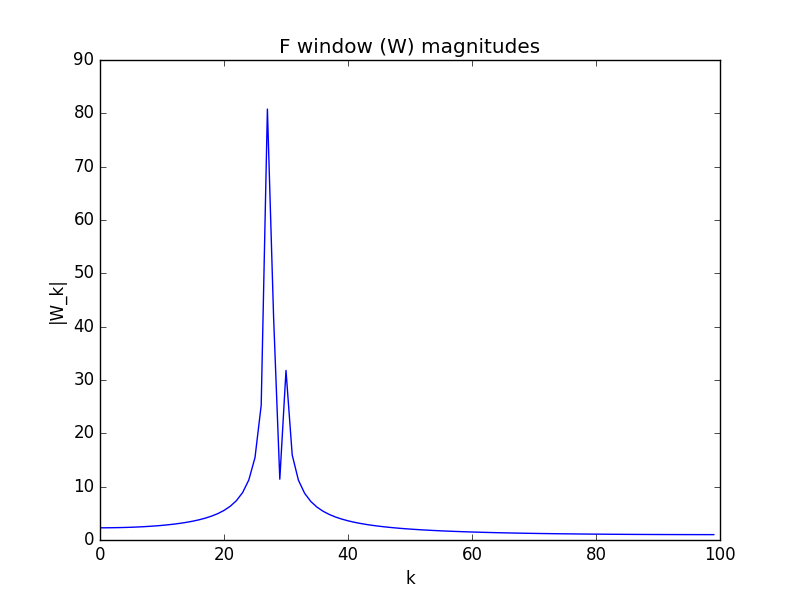
\includegraphics[width=\textwidth]{2b}
  \caption{Windowed signal magnitude plot}
  \label{fig:window}
\end{figure}
